\section{Theoretical Foundations} \label{sec:theoretical-foundations}
% \newtodo{Initial research done, looking at the existing work in the field and know the state of the art.}
% \newtodo{Keep papers for related work section which discusses alternative approaches to my solution (where background provides necessary foundations for understanding).}
% \newtodo{Introduce terminology and definitions I use. Non-trivial aspects should be mentioned here.}
% \newtodo{Introduce concepts i will use in the rest of the paper.}

This section provides the theoretical foundations for the work presented in this thesis. It covers the necessary background knowledge, including the fundamentals of \ac{llms}, the hierarchical structure of Bloom's Taxonomy, plus the various performance enhancements and evaluation methodologies.

\subsection{Understanding Large Language Models}

\object{Architectural Fundamentals} \ac{llms} -- the base of \ac{aqg} -- are commonly based on the novel neural network architecture known as transformers \cite{naik_large_2024}, released by Google \cite{vaswani_attention_2017}. It was originally proposed for machine translation \cite{minaee_large_2025,vaswani_attention_2017}. Shown in Google's paper, what makes the transformer architecture so special is that it is solely based on the attention mechanism, so it does not rely on the former approaches called \ac{rnns} or \ac{cnns}. Additionally, this architecture is capable of better parallelization, faster training times and better performance, as to be seen in its intended task \cite{vaswani_attention_2017}. Attention is essential for transformer models, allowing to model long-range dependencies effectively, but also focus and weight on important information in the input sequence \cite{patil_review_2024}. 

The transformer follows an encoder-decoder structure \cite{patil_review_2024,minaee_large_2025}. Told by \cite{minaee_large_2025,vaswani_attention_2017}, both the encoder and decoder consist of a stack of identical layers, in the original paper $N=6$ layers were used, split in two columns in the following figure.

\begin{figure}[htbp]
  \centering
   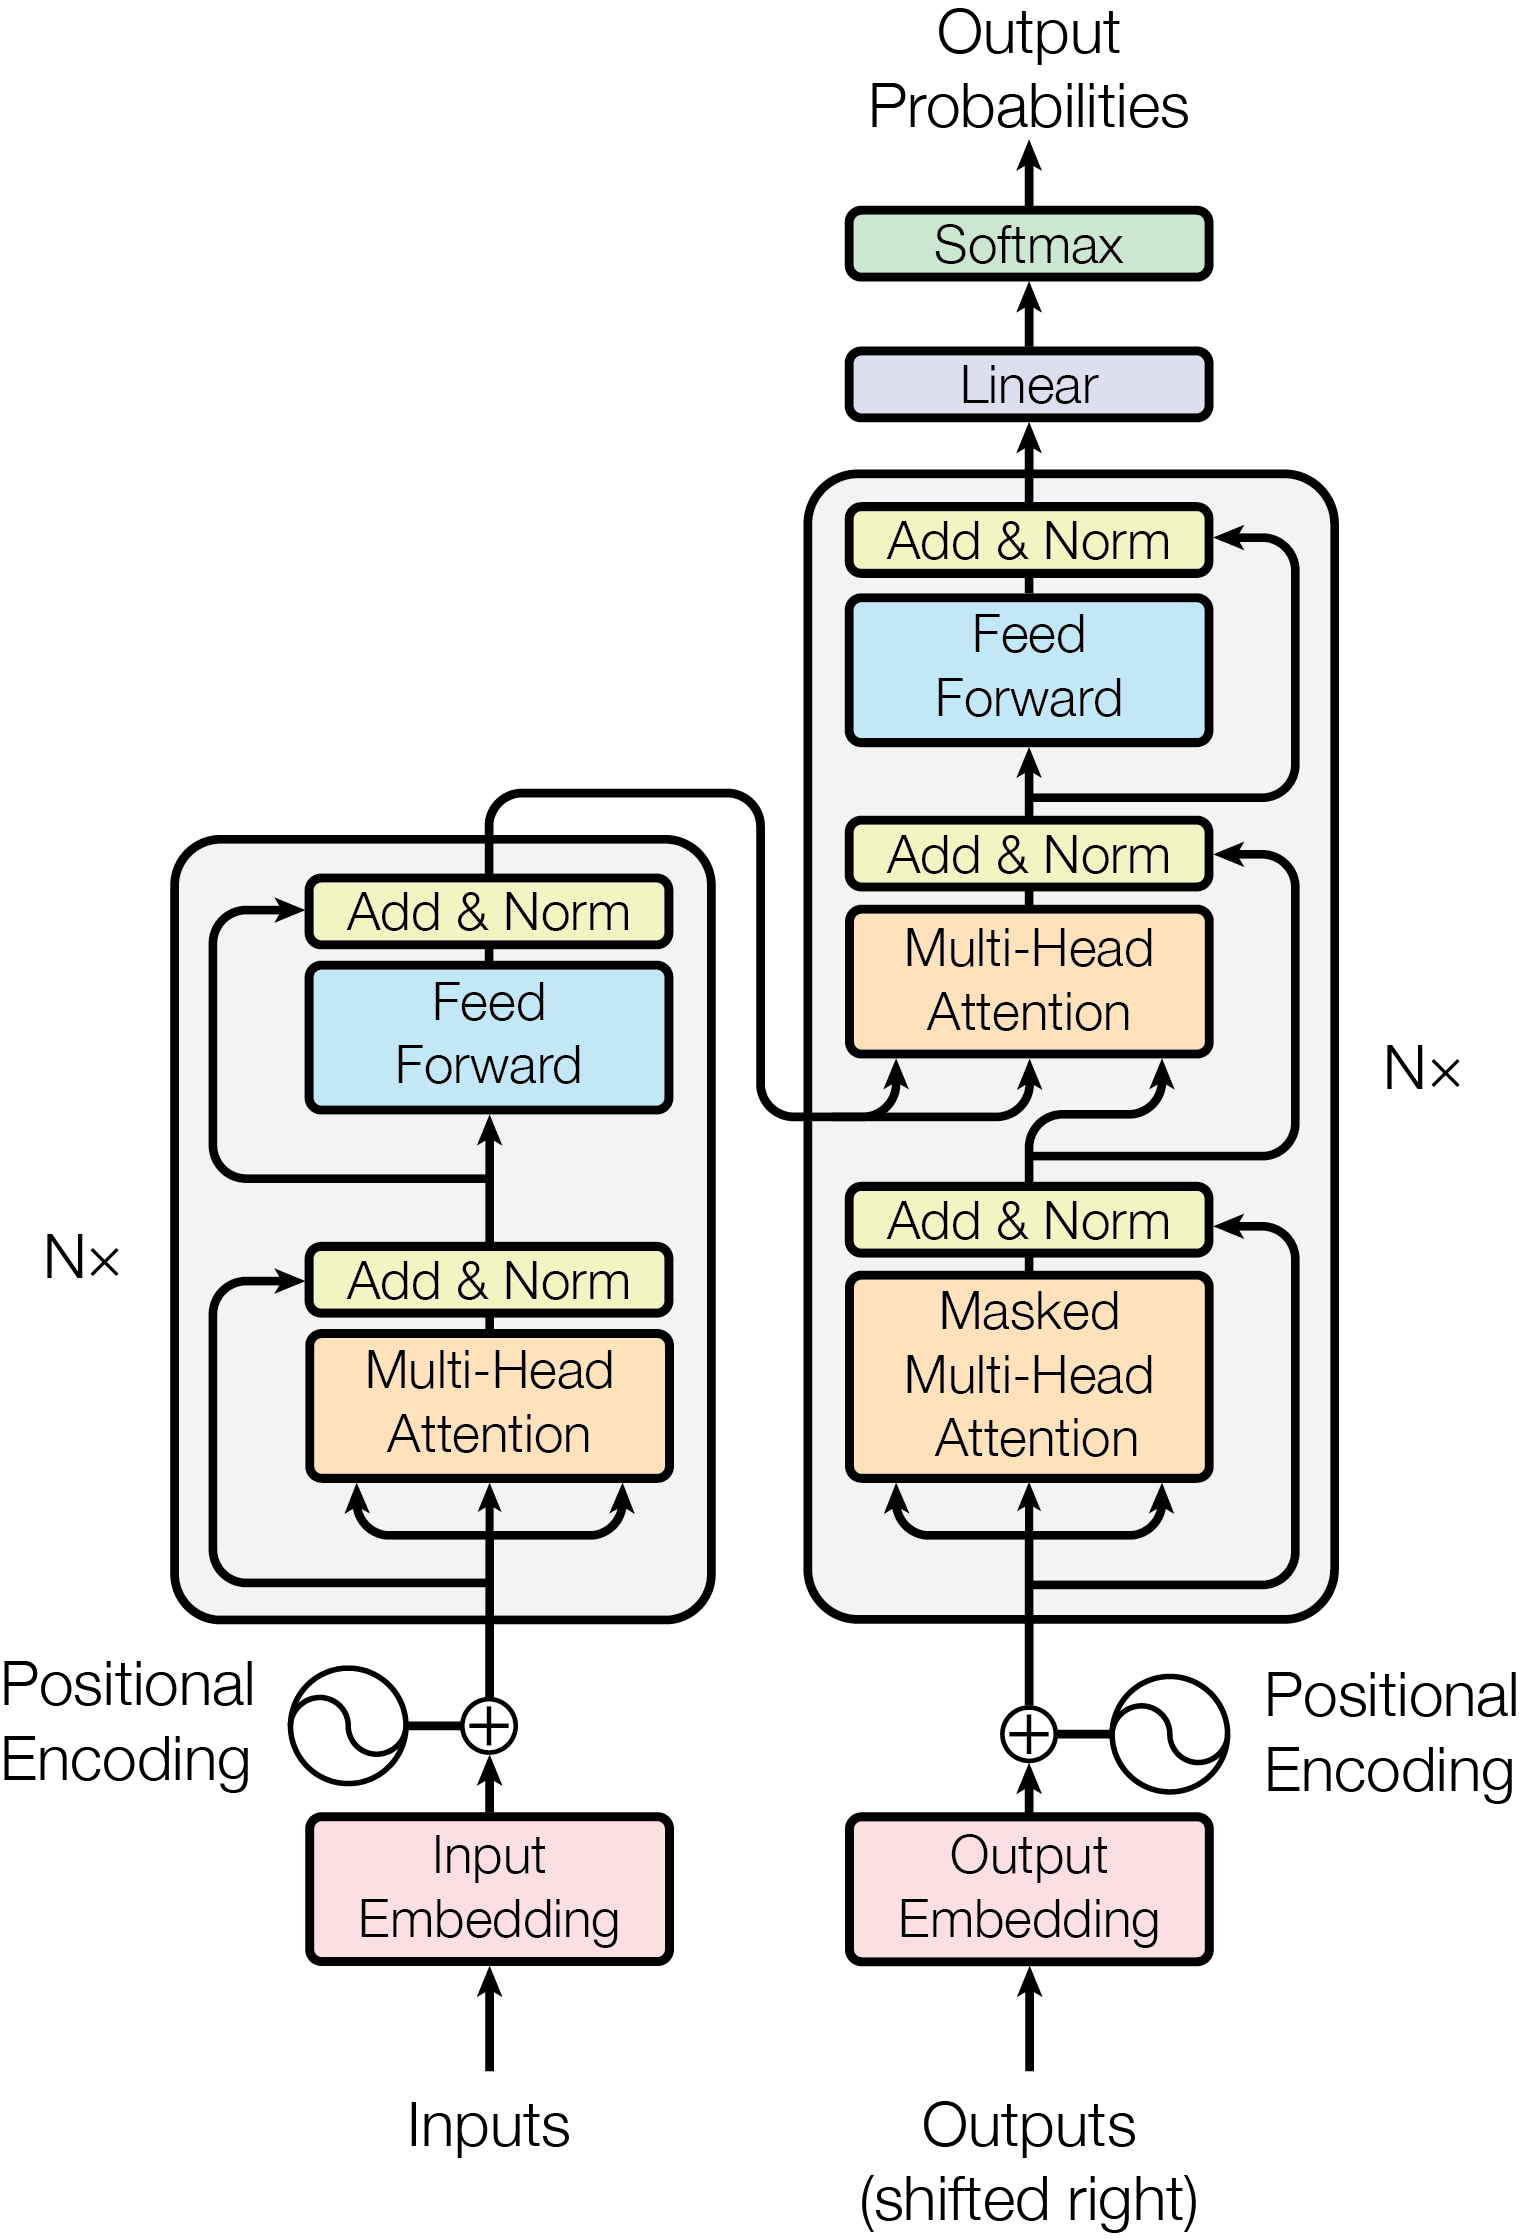
\includegraphics[width=0.4\textwidth]{../extra/transformer.png}
   \caption[Transformer Architecture.]{Transformer Architecture \cite{vaswani_attention_2017}.} 
   \label{fig:transformer-architecture}
\end{figure}

\object{Preprocessing Steps} To prepare the text for the transformer model, several steps are performed before the actual encoding and decoding process begins:

\begin{itemize}
   \item \textbf{Tokenization}. It is a crucial step for transformers and \ac{llms}, where the text is parsed into several units called tokens \cite{naveed_comprehensive_2024,raiaan_review_2024,zhao_survey_2025}, which represent characters, a group of these or words \cite{naik_large_2024}. With tokens, the next step can be performed.
   \item \textbf{Creating Embeddings}. Each token is then converted into a numeric vector representation of the same dimension \cite{vaswani_attention_2017}. By this \cite{raiaan_review_2024}, the token's meaning is mapped in a mathematical space, where comparable phrases are close together. 
   \item \textbf{Positional Encoding}. As stated in \cite{vaswani_attention_2017}, positional encoding is added to the input embeddings to provide information about the position of each token in the sequence. This is necessary because transformers do not have a built-in order, unlike \ac{rnns} or \ac{cnns}. 
\end{itemize}

\object{Left: Encoder} The encoder structure is primarily designed for processing and interpreting the input text \cite{wang_history_2024}. It extracts step-by-step features and the result is passed to the decoder \cite{liu_understanding_2024}. Each encoder layer consists of two sublayers: 

\begin{itemize}
    \item \textbf{Orange: Multi-Head Self-Attention} \cite{vaswani_attention_2017}. In this layer, every position in the input sequence can attend to all other positions in the previous layer of the encoder. By this \cite{patil_review_2024}, the model can capture dependencies between the tokens, regardless of their distance in the input sequence. 
    \item \textbf{Blue: Position-wise \ac{ffn}} \cite{vaswani_attention_2017}. This layer is applied independently to each position in the sequence. By using this layer \cite{liu_understanding_2024}, the encoder can process and extract features from the attention output.
\end{itemize}

\object{Right: Decoder} The decoder instead is responsible for generating the output sequence based on the encoded input. This results in a sequence of generated tokens \cite{raiaan_review_2024}. Each decoder layer is a bit different from the encoder layer structure. It consists of the following three sublayers:

\begin{itemize}
    \item \textbf{Orange$_1$: Masked Multi-Head Self-Attention} \cite{vaswani_attention_2017}. This layer is a modified version of the encoder's self-attention mechanism, but it prevents attending to future sequence positions. By this, the model can only use information from the past tokens and the current one.
    \item \textbf{Orange$_2$: Multi-Head Attention} \cite{vaswani_attention_2017}. This layer explicitly allows the decoder to attend over the encoder's output, enabling it to incorporate information from the input sequence.
    \item \textbf{Blue: Position-wise \ac{ffn}} \cite{vaswani_attention_2017}. This layer is similar to the one in the encoder, applied independently to each position in the sequence. In the end, the decoder output is passed to a linear layer and a softmax function to finally generate the next-token probabilities.
\end{itemize}

\pagebreak

\object{Resulting Architectures} According to the survey \cite{shao_survey_2024}, the transformer architecture has been split into three main categories, as follows:

\begin{itemize}
   \item \textbf{Encoder-only:} Earlier architectures such as Google BERT \cite{devlin_bert_2019} and its derivates, e.g.\ Huawei ERNIE \cite{zhang_ernie_2019}, Meta RoBERTa \cite{liu_roberta_2019} and Google ALBERT \cite{lan_albert_2020} are solely based on the encoder component. This results a niche for these models being suitable for specific \ac{nlp} tasks focused on comprehension. According to the survey \cite{hou_large_2024}, these models process and encode input into hidden representations to capture word relationships and contextual information. Here, models like BERT observe both the left and right context of the currently focused word.
   
   \item \textbf{Decoder-only}:
   More current models e.g.\ Meta's LLaMA series \cite{touvron_llama_2023}, OpenAI's GPT-1 \cite{radford_improving_2018} to GPT-4 \cite{openai_gpt-4_2024}, and ChatGPT \cite{openai_introducing_2022}, focus on token generation based solely on the preceding tokens \cite{shao_survey_2024}. According to \cite{hou_large_2024}, without the reliance on the encoder, decoder-only transformers can be used for diverse generation tasks, such as code generation and code completion.

   \item \textbf{Encoder-Decoder}: Certain architectures such as Google's T5 \cite{raffel_exploring_2023} and their BART model \cite{lewis_bart_2019} integrate both the encoder and decoder components. This leads to hybrid capabilities, combining the understanding of the input and the proper generation of the output. According to \cite{wang_history_2024}, these models are applicable to e.g.\ machine translation, text summarization and question answering. However, the complexity of the dual architecture can lead to demanding training processes and slower inference times.
\end{itemize}

\object{\ac{moe}} Another notable variant of the transformer architecture is the \ac{moe} \cite{shazeer_outrageously_2017} architecture, as shown in the overview by \cite{naveed_comprehensive_2024}. In this architecture, multiple experts are integrated. Typically, an \ac{moe} system is a mixture of an \ac{ffn} for each expert, positioned right after the attention block, and a router mechanism, which decides which token(s) are processed by which expert(s). These are advantageous in terms of computational efficiency while being as powerful as dense models. That means, the size of the model can be increased without increasing the computational cost proportionally, because only a subset of the experts is activated for each input. % [91,92]
 Prominent examples of \ac{moe} models are xAI Grok-1 \cite{xai_open_2024}, Gemini 1.5 by Google \cite{team_gemini_2024-1}, the DeepSeek models V3 \cite{deepseek-ai_deepseek-v3_2025} and its reasoning variant R1 \cite{deepseek-ai_deepseek-r1_2025}, and the recently released LLaMA 4 family by Meta \cite{meta_ai_llama_2025}.

\vp

\subsection{Framing Bloom's Taxonomy for LLM Applications} \label{sec:blooms-taxonomy}

Given \ac{llms}' capabilities, these enable the automation of the often time-consuming question generation process for educators \cite{vu_chatgpt-based_2024}. The integration of such models into education offers an opportunity to enhance the learning experience for students and support teachers in advancing educational content \cite{naveed_comprehensive_2024}. 
With the help of \ac{llms}, customized study materials and practice questions can be generated to develop personalized learning for students \cite{al_faraby_analysis_2024,bhowmick_automating_2023,hang_mcqgen_2024}, while freeing up the educators' valuable time for both teaching and student interaction \cite{naveed_comprehensive_2024}.
% sources: 452 part 1 / 453.454 for part 2 
% Diverse and inclusive materials can be created with the help of \ac{llms}, thereby freeing up valuable time for both teaching and student interaction \cite{naveed_comprehensive_2024}. 
% However, aligning the automated questions with specific cognitive levels still remains a key challenge. 

\object{Challenge of Alignment} For automated content creation and personalized learning, the ability to differentiate questions based on certain levels of cognitive complexity is crucial \cite{li_planning_2024,zhuge_twinstar_2025}. However, aligning the automated questions with specific cognitive levels still remains a key challenge. \ac{llms} per se show great potential in \ac{aqg} with respect to different cognitive levels \cite{maity_can_2025,blobstein_angel_2023,duong-trung_bloomllm_2024,scaria_automated_2024,scaria_how_2024}. By using different prompting strategies, as illustrated in the \bfhyperref{sec:performance-enhancements}{Performance Enhancements} and the according \bfhyperref{sec:question-generation-research}{Question Generation Research} section, the models can be guided to generate questions that are aligned with the cognitive levels of Bloom's Taxonomy. Certain approaches can generate questions across all levels of Bloom's Taxonomy \cite{duong-trung_bloomllm_2024,zhuge_twinstar_2025}. However, despite their proficiency at lower levels, \ac{llms} occasionally struggle with adherence at the higher levels \cite{duong-trung_bloomllm_2024,cheng_treequestion_2024,elkins_how_2023}.

\object{Cognitive Hierarchy} In the academic literature, Bloom's Taxonomy \cite{krathwohl_taxonomy_1964} and primarily its revised version \cite{krathwohl_revision_2002} are often discussed in the context of question generation and evaluation with respect to \ac{llms} \cite{zhuge_twinstar_2025,scaria_automated_2024,scaria_how_2024,elkins_how_2023}.
According to \cite{krathwohl_revision_2002}, this taxonomy follows a hierarchical structure where the six main categories are organized by increasing complexity, with each level building upon a less complex predecessor excepting the lowest level. The following figure\footnote{\url{https://citt.ufl.edu/resources/the-learning-process/designing-the-learning-experience/blooms-taxonomy/blooms-taxonomy-graphic-description/}, accessed 04/29/2025} shows the cognitive levels of Bloom's Taxonomy in its revised version.

\begin{figure}[htbp]
   \vspace{-.5em}
   \centering
   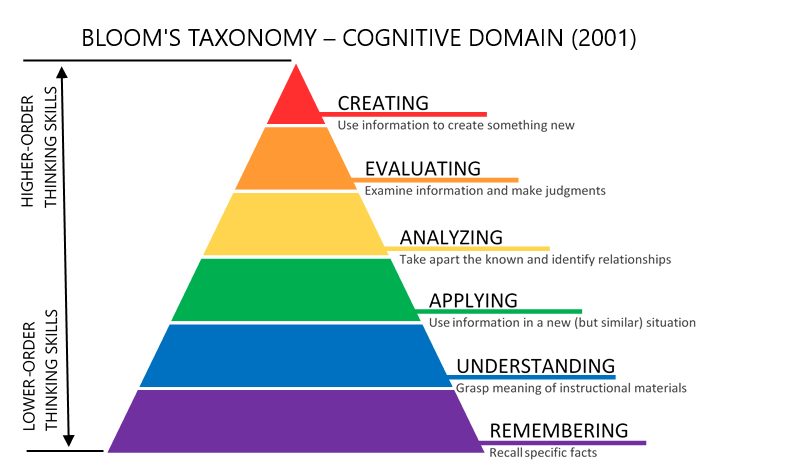
\includegraphics[width=0.65\textwidth]{../extra/Blooms-Taxonomy.png}
   \caption{Hierarchy of Bloom's Revised Taxonomy.}
\end{figure}

The revised taxonomy \cite{krathwohl_revision_2002} is divided into six levels. Each level is associated with a specific cognitive skill, as follows with ascending complexity:

\begin{itemize}
   \item \textbf{Remembering:} Formerly known as \enquote{Knowledge}, this level refers to the retrieval of relevant knowledge from long-term memory by focusing on recognition and recall of facts.
   \item \textbf{Understanding:} This level, previously called \enquote{Comprehension}, involves identifying the meaning of instructional messages, such as oral, written and graphic communication.
   \item \textbf{Applying:} This level is about carrying out or using a procedure in a given situation.
   \item \textbf{Analyzing:} This involves breaking down material into its components and determining their relationships to one another or to an overall structure or purpose.
   \item \textbf{Evaluating:} This level requires making judgements based on established criteria and standards.
   \item \textbf{Creating:} This is the highest cognitive level and involves assembling or reorganizing elements into a coherent whole.
\end{itemize}

Each of these cognitive levels is associated with a set of action verbs that can be used to formulate learning objectives and assessment questions. A comprehensive list of such verbs, categorized by these cognitive levels, can be found at the University of Arkansas' website\footnote{\url{https://tips.uark.edu/blooms-taxonomy-verb-chart/}, accessed 05/13/2025}. The following table offers a brief overview of the cognitive levels and their corresponding action verbs:

% Du meinst ja oben, dass diese Taxonomy schon genutzt wird, um die Relevanz von LLMs zu untersuchen. Wenn das stimmt, dann würde ich dir empfehlen, hier auch Forschungsbefunde zusammenzufassen. Also was haben die schon untersucht und wo gibt es Forschungslücken, die du jetzt adressieren möchtest

\begin{table}[htbp]
   \centering
   \renewcommand{\arraystretch}{1.6} % Matches row height style from the example table
   \caption{Bloom's Taxonomy Action Verbs.}
   \label{tab:blooms_verbs_columns}
   \begin{tabularx}{\textwidth}{|>{\hsize=1.15\hsize\centering\arraybackslash}X|>{\hsize=1.25\hsize\centering\arraybackslash}X|>{\hsize=0.95\hsize\centering\arraybackslash}X|>{\hsize=0.95\hsize\centering\arraybackslash}X|>{\hsize=0.9\hsize\centering\arraybackslash}X|>{\hsize=0.8\hsize\centering\arraybackslash}X|}
     \hline
     \rowcolor{gray!15}
     \textbf{Remembering} & \textbf{Understanding} & \textbf{Applying} & \textbf{Analyzing} & \textbf{Evaluating} & \textbf{Creating} \\
     \hline
     Define & Clarify & Apply & Analyze & Assess & Assemble \\
     \hline
     Describe & Classify & Calculate & Break down & Conclude & Code \\
     \hline
     Enumerate & Compare & Demonstrate & Detect & Criticize & Compile \\
     \hline
     Identify & Contrast & Determine & Differentiate & Defend & Construct \\
     \hline
     List & Detail & Examine & Distinguish & Evaluate & Create \\
     \hline
     Match & Explain & Illustrate & Examine & Grade & Design \\
     \hline
     Name & Paraphrase & Modify & Investigate & Interpret & Develop \\
     \hline
     Outline & Rewrite & Simulate & Optimize & Judge & Enhance \\
     \hline
     Quote & Summarize & Solve & Relate & Justify & Improve \\
     \hline
     Select & Translate & Use & Separate & Verify & Reorganize \\
     \hline
   \end{tabularx}
 \end{table}

\pagebreak

\subsection{Performance Enhancements}
\label{sec:performance-enhancements}

To address these challenges and to refine the capabilities of \ac{llms} for specific tasks, such as \ac{aqg}, various performance enhancement strategies have been proposed. These techniques aim to improve the quality and relevance of the generated content, as listed in the following:

\object{In-Context Learning} As highlighted by \cite{zhao_survey_2025}, the advent of GPT-3 \cite{brown_language_2020} introduced the concept of in-context learning. OpenAI further delineated this into subcategories such as zero-shot, one-shot, and few-shot learning, depending on how many examples are provided in the prompt.

\object{\ac{cot}} This technique, introduced by \cite{wei_chain--thought_2022}, enhances in-context learning by prompting reasoning steps to elicit the \ac{llms}' step-by-step reasoning \cite{zhao_survey_2025}. Moreover, this method can lead to higher quality questions \cite{scaria_automated_2024}, as depicted in \cite{wei_chain--thought_2022}.

\object{Role-based Prompting} This technique involves assigning a specific role or persona to the model while prompting it \cite{zhao_survey_2025} to better fulfill the task instruction. The advantages of the approach are further discussed in the according paper \cite{kong_better_2024} independently of the survey paper.

\object{Self-Refinement} By iteratively refining the \ac{llm}-generated output based on feedback \cite{madaan_self-refine_2023}, the overall process and the corresponding solutions can be improved \cite{zhao_survey_2025}.

\object{Using Special Marks} Emphasizing important parts of the prompt can be achieved by using special marks like quotation marks or line breaks \cite{zhao_survey_2025} to help the \ac{llm} visually distinguish between different parts of the prompt. 

\object{Positive Constraints} When formulating the prompt, it is often more useful to tell the model what it should do, rather than what it should not do \cite{zhao_survey_2025}. 

\object{Providing Scoring Standards} For tasks which involve scoring a text, it is crucial to provide a detailed description of the scoring standards in the prompt \cite{zhao_survey_2025}. For instance, this clear rubric helps the \ac{llm} to assess the quality of generated questions \cite{scaria_automated_2024}.

\object{\ac{rag}} This method \cite{lewis_retrieval-augmented_2020}, as used in approach \cite{hang_mcqgen_2024}, highlights how external knowledge sources can be integrated at \ac{aqg} prompts. For this, querying a comprehensive database is needed to retrieve relevant information that is useful the context of the question. This can be realized via e.g.\ knowledge graphs as domain-specific knowledge, which can be based on course content \cite{yang_heuristic_2024}.

\object{Model Fine-Tuning} A key strategy to adapt general-purpose \ac{llms} to specific tasks by training them on domain-specific data \cite{hou_large_2024}. By this process, models can learn knowledge relevant to a specific context, aber traditional full fine-tuning requires vast amounts of data and computational resources \cite{hou_large_2024}. For instance, \cite{duong-trung_bloomllm_2024} fine-tuned their \ac{aqg} model with more than 1000 questions, which is a relatively small amount of data.

\object{Integration of Contextual Knowledge} Several studies \cite{biancini_multiple-choice_2024,blobstein_angel_2023,wang_towards_2022,bhowmick_automating_2023} have injected topic-related contextual information directly into the prompt to avoid hallucinating and give users control over the source of knowledge \cite{biancini_multiple-choice_2024}.

\vp

\subsection{Evaluation Methodologies}

Evaluation is always necessary to assess the quality of LLMs for the task at hand. According to \cite{doughty_comparative_2024}, evaluating automatically generated learning resources is important because they often lack the deep qualities necessary for their effectiveness.
The methods to evaluate \ac{llms} at e.g.\ \ac{aqg} can be divided into several categories:

\object{$\mathbf{n}$-gram-based Metrics} These metrics follow a reference-based approach, where the generated text is compared to a reference text. The evaluation is based on the overlap of sequences of $n$ words between the generated and reference text \cite{guo_survey_2024}. The most common metrics in this category are:
\begin{itemize}
   \item \textit{\ac{bleu}} \cite{papineni_bleu_2001} evaluates the average $n$-gram precision against a reference text, so how many $n$-grams from the generated text are also present in the reference text \cite{guo_survey_2024}.
   \item \textit{\ac{rouge}}, proposed by \cite{lin_rouge_2004}, calculates recall, which is the ratio of $n$-grams from a ground truth text that are also present in the generated text \cite{guo_survey_2024}.
   \item \textit{\ac{meteor}} \cite{banerjee_meteor_2005} calculates the harmonic mean of precision and recall, so it provides a balanced evaluation \cite{guo_survey_2024}.
\end{itemize}

% -------------------------------------------------------------------------

\object{Diversity-based Metric} The more recent \textit{Distinct-}$n$ \cite{li_diversity-promoting_2016} measures text diversity by calculating the proportion of unique $n$-grams, though it is considered overly simplistic \cite{guo_survey_2024}.

% -------------------------------------------------------------------------

\object{Semantic Similarity} Metrics in this category assess sentence-level comparison, which is vital beyond word-level comparisons \cite{guo_survey_2024}.
\begin{itemize}
   \item \textit{BERTScore} \cite{zhang_bertscore_2020} compares contextual sentence-level embedding vectors from a pre-trained BERT model by calculating cosine similarity between the embeddings of the generated and reference text \cite{guo_survey_2024}.
   \item Manual cosine similarity calculation can also be calculated by comparing embeddings created by an embedding model, as it was done in \cite{li_planning_2024}.
\end{itemize}

\object{Other Metrics} Apart from these categories, diverse other methods and metrics are used to evaluate the generated questions:

\begin{itemize}
   \item For instance, \cite{wang_towards_2022} assessed question quality using \textit{Perplexity} (via GPT-2 \cite{radford_language_2019}), \textit{Diversity} (Distinct-3 score \cite{li_diversity-promoting_2016}), \textit{Toxicity, Grammatical Error,} and the resulting \textit{Acceptability} of a question. \cite{yang_heuristic_2024} also adopted \textit{Perplexity, Diversity,} and \textit{Toxicity}.
   \item Additionally, researchers developing new evaluation metrics often compare their approaches against a range of existing ones. For example, \cite{nguyen_reference-based_2024} benchmarked their proposed metric against \textit{BLEU, ROUGE, BERTScore, QAScore} -- predicting answer extractability from the given context via transformers -- \cite{ji_qascoreunsupervised_2022}, Google's \textit{\ac{bleurt}} -- predicting human judgements of text quality -- \cite{sellam_bleurt_2020}, and the also BERT-based \textit{\ac{rquge}} metric by Meta -- comparing predicted and gold answer spans -- \cite{mohammadshahi_rquge_2023}.
\end{itemize}

% -------------------------------------------------------------------------

\object{Knowledge Graphs} The authors \cite{luo_systematic_2023} presented a framework leveraging knowledge graphs with facts to systematically assess the factual knowledge of LLMs. Frameworks like this can be used to generate questions and their expected answers from given knowledge graph triplets -- such as \texttt{<subject, relation label, object>} -- to evaluate the \ac{llm}'s accuracy.

% -------------------------------------------------------------------------

\object{Human Evaluation} This kind of evaluation is considered necessary to judge about the quality of generated questions \cite{horbach_linguistic_2020}.

\begin{itemize}
   \item While criticizing former used metrics such as \textit{BLEU} and \textit{METEOR} not covering a proper evaluation on question quality, \cite{horbach_linguistic_2020} presented a novel hierarchical evaluation scheme for question generation to guide the human annotators. The scheme often considers binary choices, to induce clear decisions. The following 9 criteria were presented: \textit{Understandable, DomainRelated, Grammatical, Clear, Rephrase, Answerable, InformationNeeded, Central, WouldYouUseIt}. 
   \item Studies such as \cite{steuer_i_2021} and \cite{moore_assessing_2022} adopted this hierarchical scheme and used it for their human question evaluation. For instance, \cite{steuer_i_2021} used it to evaluate their \ac{aqg} system, while \cite{moore_assessing_2022} adopted this scheme to assess the quality of student-generated questions.
   \item Furthermore, the authors in the papers \cite{scaria_how_2024,scaria_automated_2024} used and adapted the evaluation scheme by replacing the criterion \textit{Rephrase} with \textit{Bloom'sLevel}.
   \item  Using \cite{moore_assessing_2022} as a reference, \cite{mi_comparative_2024} proposed another scheme with a maximum of 50 points by covering \textit{Relevance, Clarity, Answerability, Challenging} and \textit{Cognitive Level} as criteria. The latter results in a higher score for questions that are more cognitively demanding, so higher in the Bloom's Taxonomy hierarchy. GPT-4 had most voting agreement with expert ratings in contrast to e.g.\ GPT-3.5 and ERNIE.
   \item Moreover, \cite{moore_automatic_2024} proposed a novel evaluation toolkit for question usability, called SAQUET. Using the 19-item writing flaw rubric by \cite{tarrant_frequency_2006}, they evaluated the \ac{mcqs}. Based on these criteria, the structural and pedagogical value of the questions was assessed, with SAQUET being slightly more strict at rating than the experts.
\end{itemize}

% -------------------------------------------------------------------------

\object{LLM as an evaluator} Another approach involves using \ac{llms} themselves as evaluators. For instance, \cite{nguyen_reference-based_2024} introduced NACo, an \ac{llm}-based metric that employs a \ac{cot} strategy to rank the \textit{Naturalness, Complexity} and \textit{Answerability} of generated questions. In contrast to this, \cite{scaria_how_2024} employed Gemini Pro\footnote{\url{https://blog.google/technology/ai/google-gemini-ai/\#performance}, accessed 05/09/2025} to assess \textit{Question Quality} and \textit{Alignment} with Bloom's Taxonomy, revealing discrepancies compared to human evaluators. It is noteworthy that the abilities of \ac{llms} are rapidly evolving, and results from former models, e.g.\ Gemini Pro, might differ with versions nowadays. 

Other research has also explored using \ac{llms} for tasks like classifying question quality, evaluating answerability, or performing other evaluations based on predefined criteria \cite{moore_assessing_2022,scaria_how_2024,blobstein_angel_2023}. The use of \ac{llms} for evaluation is a promising direction, especially when coupled with human evaluation. Comparing the agreement between the \ac{llm} and the experts can enhance the reliability of the evaluation process.
